%%%%%%%%%%%%%%%%%%%%%%%%%%%%%%%%%%%%%%%%%%%%%%%%%%%%%%%%%%%%%%%%%%%%%%%%%%%%%%%
% Chapter 3: Procedimiento experimental 
%%%%%%%%%%%%%%%%%%%%%%%%%%%%%%%%%%%%%%%%%%%%%%%%%%%%%%%%%%%%%%%%%%%%%%%%%%%%%%%

%++++++++++++++++++++++++++++++++++++++++++++++++++++++++++++++++++++++++++++++
\section{Descripci�n de los experimentos}
\label{3:sec:1}

Vamos a aplicar la regla del trapecio a la funci�n sin(pi*x) en el intervalo [-2,-1] utilizando una cantidad variable de subintervalos, n. Para cada valor de n, mediremos el error absoluto y el tiempo de ejecuci�n del m�todo. Adicionalmente, aplicaremos la regla de Simpson a la misma funci�n con iguales par�metros para comparar ambos m�todos.

%++++++++++++++++++++++++++++++++++++++++++++++++++++++++++++++++++++++++++++++
\section{Descripci�n del material}
\label{3:sec:2}

Los experimentos han tenido lugar sobre un procesador Intel Core i3-2350M a 2.30 GHz. N�tese que aunque la m�quina tiene cuatro procesadores, s�lo se emple� uno para realizar los c�lculos. El sistema operativo fue Linux Mint 14.1 (Nadia) con la versi�n 3.5.0-17 del kernel. Los algoritmos fueron implementados en Python y la versi�n del int�rprete fue la 2.7.3.

%++++++++++++++++++++++++++++++++++++++++++++++++++++++++++++++++++++++++++++++
\section{Resultados obtenidos}
\label{3:sec:3}

Aqu� vamos a esperar hasta tener la tabla resumen, las gr�ficas y el c�lculo anal�tico de la cota del error.
%------------------------------------------------------------------------------
\begin{figure}[!th]
\begin{center}
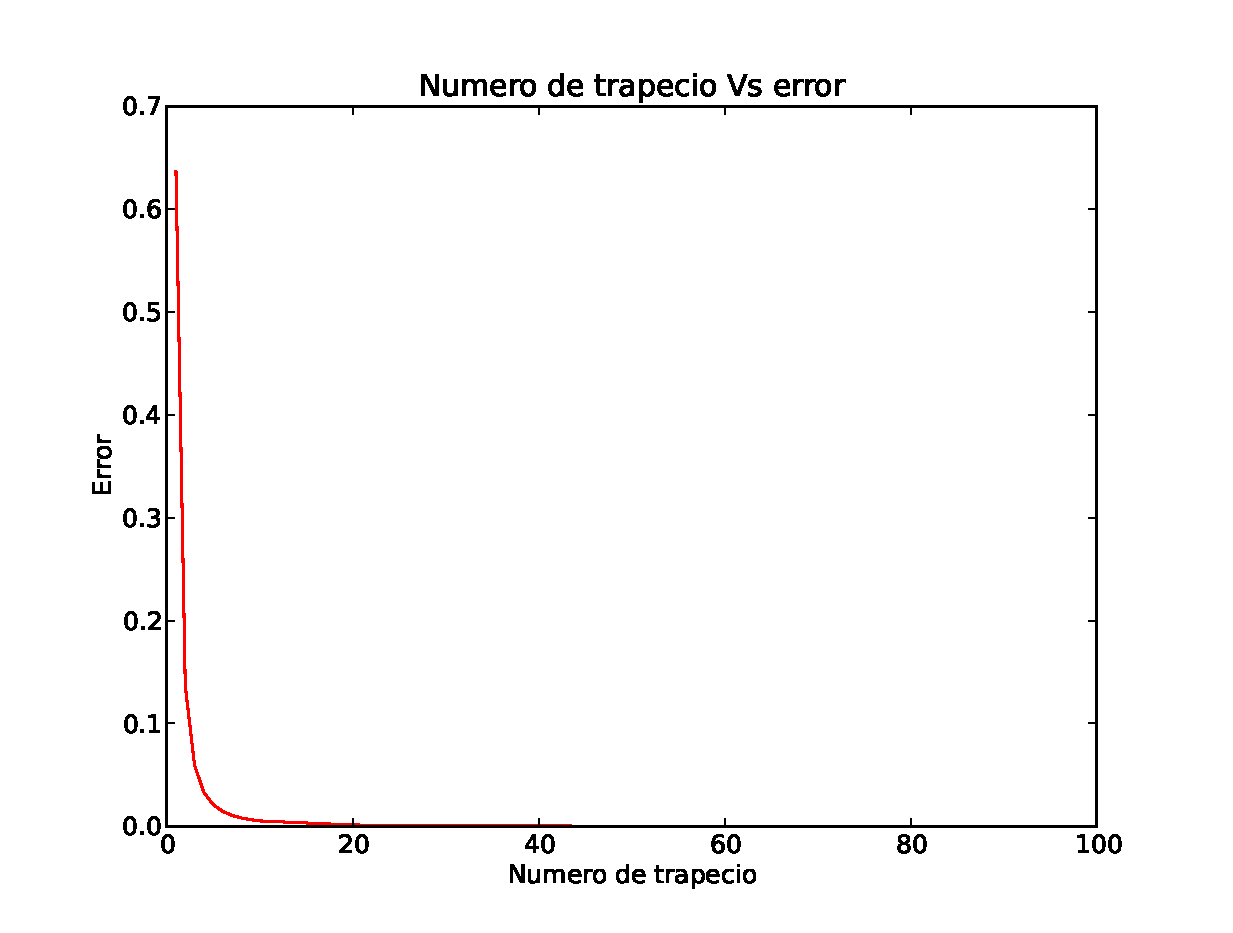
\includegraphics[width=0.75\textwidth]{img/Plot_nVSerror.eps}
\caption{nVSerror}
\label{fig:1}
\end{center}
\end{figure}
%------------------------------------------------------------------------------
\begin{figure}[!bh]
\begin{center}
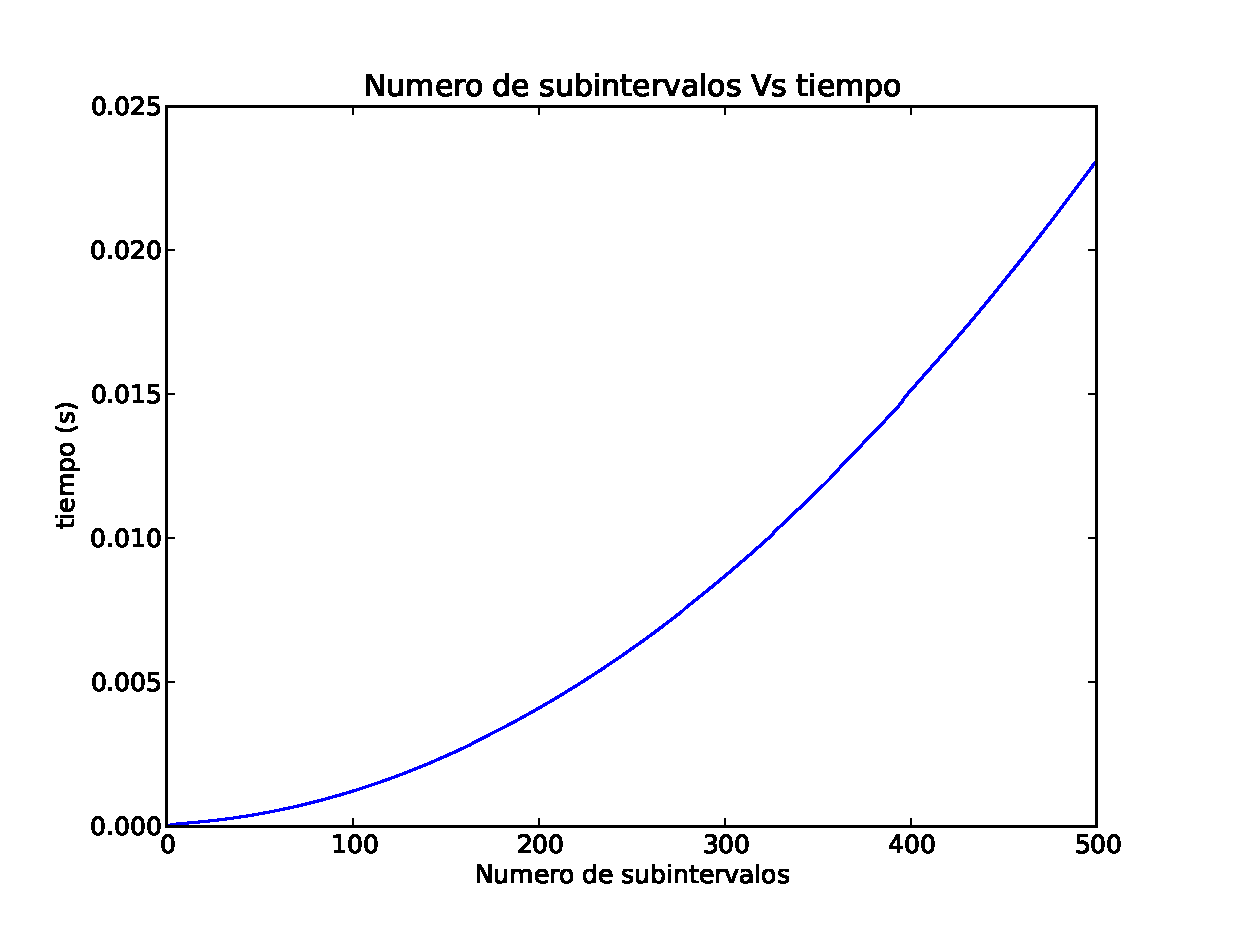
\includegraphics[width=0.75\textwidth]{img/Plot_nVStime.eps}
\caption{nVStiempo}
\label{fig:2}
\end{center}
\end{figure}
%------------------------------------------------------------------------------

\DTLloaddb[noheader,keys={n,error,tiempo}]{table1}{mydata.csv}
\newcolumntype{d}{D{,}{\pm}{-1}} 

\begin{table}[!h]
 \begin{center}
  \begin{tabular}{l|c|r}% 
    {\bf n} & {\bf error} & {\bf tiempo}
    \DTLforeach*{table1}{%
      \n=n,\error=error,\tiempo=tiempo}{%
      \\
      \n & \error & \tiempo}%
  \end{tabular}
  \caption{Resultados optenidos por número de trapecios}
  \label{tabla:1}
  \end{center}
\end{table}                                     

%------------------------------------------------------------------------------


%++++++++++++++++++++++++++++++++++++++++++++++++++++++++++++++++++++++++++++++
\section{An�lisis de los resultados}
\label{3:sec:4}

bla, bla, etc. 

